\chapter{质点系；刚体入门}\label{ch:b1:systems-of-points}

跳水运动员离开跳板，蜷身，翻转两周，然后伸直身体；
在整个过程中，她身体上的一点——她的\omterm{def:b1:systems-of-points:cm}{质心}——
所走的\omterm{def:b1:point-kinematics:frame}{轨迹}与石头相同，都是一条普通的抛物线。从手中释放的溜溜球
到达绳子末端所用的时间是石头的三倍，
并以每分钟两千转的转速旋转着到达。一个
实心球沿任何斜面滚下都快于空心球，无论两者的大小
或质量如何。前面几章中单个质点的力学，
可以推广到由许多质点组成的系统——以及日常生活中的\omterm{def:b1:systems-of-points:solid}{刚体}——
依靠若干定理：\omterm{def:b1:systems-of-points:cm}{质心}
如同一个质点那样运动，能量与\omterm{def:b1:angular-momentum:L}{角动量}分解为\omterm{def:b1:systems-of-points:cm}{质心}部分与
“围绕”\omterm{def:b1:systems-of-points:cm}{质心}的部分，\omterm{def:b1:systems-of-points:solid}{绕定轴转动}的\omterm{def:b1:systems-of-points:solid}{刚体}是
一个单自由度系统，由其\omterm{prop:b1:angular-momentum:inertia}{转动惯量}决定。

\section{质心与动量}

\begin{definition}[质心；质点系的动量]\label{def:b1:systems-of-points:cm}
\index{质心}\index{质心}
设各质点的质量为 $m_i$，位于 $M_i$ 处，总质量 $M = \sum m_i$，
则\emph{质心} $G$ 由下式定义
\[
\sum_i m_i\,\vect{GM_i} = \vect 0, \qquad\text{即}\qquad
\vect{OG} = \frac{1}{M}\sum_i m_i\,\vect{OM_i}
\]
对任意原点 $O$ 成立。质点系的\emph{动量}为 $\vect P =
\sum_i m_i\vect v_i = M\vect v_G$。
\end{definition}

\begin{theorem}[质心定理]\label{thm:b1:systems-of-points:cmtheorem}
\index{质心定理}\index{动量守恒}
在\omterm{thm:b1:newton-dynamics:laws}{惯性参考系}中，
\[
M\,\vect a_G = \frac{\dd\vect P}{\dd t} = \sum\vect F_{\mathrm{ext}} :
\]
\omterm{def:b1:systems-of-points:cm}{质心}的运动如同一个质量为 $M$ 的质点，
只受\emph{外力}的合力作用。对于\omterm{def:b1:newton-dynamics:conservation}{封闭系统}，
即无外力时，$\vect P$ 守恒，$G$ 做匀速运动。
\end{theorem}

\begin{proof}
对各质点的牛顿第二定律求和，内力两两相消，
因作用力与反作用力成对出现；由 $\sum m_i\vect a_i = M\vect a_G$
对 $G$ 的定义式求两次导数即得。
\end{proof}

\begin{example}[跳水、反冲与碰撞]\label{ex:b1:systems-of-points:cm}
\index{碰撞}
跳水运动员的 $G$ 仅在重力作用下沿抛物线运动，无论她
如何扭转——她的肌肉作用力均为内力。一支 \qty{4.0}{kg} 的步枪
发射一颗 \qty{10}{g} 的子弹，速度为 \qty{800}{m/s}：发射前后 $\vect P = \vect 0$，
故步枪以 \qty{2.0}{m/s} 的速度后坐。两辆汽车，一辆质量为 \qty{1000}{kg}
速度为 \qty{20}{m/s}，另一辆质量为 \qty{1500}{kg} 且静止，两车碰后粘在一起：$v =
20000/2500 = \qty{8.0}{m/s}$——\omterm{def:b1:newton-dynamics:conservation}{动量守恒}，而 $60\%$ 的
\omterm{thm:b1:work-and-energy:ke}{动能}转化为金属形变与热量。动量在
每次碰撞中均守恒；\omterm{thm:b1:work-and-energy:ke}{动能}只在\emph{弹性}碰撞中守恒
（见\cref{exo:b1:systems-of-points:12}）。
\end{example}

\section{柯尼希定理}

\begin{definition}[质心参考系]\label{def:b1:systems-of-points:barycentric}
\index{质心参考系}
\emph{\omterm{def:b1:systems-of-points:cm}{质心}\omterm{def:b1:point-kinematics:frame}{参考系}} $\mathcal R^*$ 的原点位于 $G$，
与\omterm{thm:b1:newton-dynamics:laws}{惯性参考系} $\mathcal R$ 作平动（其坐标轴
方向保持不变）。在其中测得的量加星号：$\vect v_i^*
= \vect v_i - \vect v_G$，且 $\sum m_i\vect v_i^* = \vect 0$。
\end{definition}

\begin{theorem}[柯尼希定理]\label{thm:b1:systems-of-points:koenig}
\index{柯尼希定理}
质点系对点 $O$ 的\omterm{def:b1:angular-momentum:L}{角动量}与\omterm{thm:b1:work-and-energy:ke}{动能}，
可分解为\omterm{def:b1:systems-of-points:cm}{质心}的贡献（\omterm{def:b1:systems-of-points:cm}{质心}携带全部质量）与
\omterm{def:b1:systems-of-points:barycentric}{质心参考系}中的贡献之和：
\[
\vect L_O = \vect{OG}\wedge M\vect v_G + \vect L^*, \qquad
E_k = \tfrac12 Mv_G^2 + E_k^*,
\]
其中 $\vect L^* = \sum\vect{GM_i}\wedge m_i\vect v_i^*$ 与 $E_k^* = \sum\tfrac12
m_iv_i^{*2}$ 均与\omterm{def:b1:point-kinematics:frame}{参考系}原点的选取无关。
\end{theorem}

\begin{proof}
利用 $\vect{OM_i} = \vect{OG} + \vect{GM_i}$ 与 $\vect v_i = \vect v_G + \vect v_i^*$，
展开 $\sum\vect{OM_i}\wedge m_i\vect v_i$ 与 $\sum\tfrac12 m_iv_i^2$：交叉项
含 $\sum m_i\vect{GM_i} = \vect 0$ 或 $\sum m_i\vect v_i^* = \vect 0$，
均为零。
\end{proof}

\begin{example}[滚动的车轮]\label{ex:b1:systems-of-points:rolling}
\index{纯滚动}
一个质量为 $M$、半径为 $R$、绕其轴的\omterm{prop:b1:angular-momentum:inertia}{转动惯量}为 $J$ 的车轮，
以速率 $v$ 做\omterm{ex:b1:systems-of-points:rolling}{纯滚动}：接触点静止，因此
$\omega = v/R$，且 $E_k = \tfrac12 Mv^2 + \tfrac12 J\omega^2 = \tfrac12 Mv^2(1 +
J/MR^2)$——对匀质圆盘，\omterm{thm:b1:work-and-energy:ke}{动能}为 $Mv^2$ 的四分之三（$J = \tfrac12 MR^2$），
对圆环则为 $Mv^2$。第二项正是自行车车轮要做得
轻的原因：其转动要耗费能量，而车架的质量则不然。
\end{example}

\section{二体问题}

\begin{proposition}[约化质量]\label{prop:b1:systems-of-points:twobody}
\index{二体问题}\index{约化质量}
两个仅相互作用的质点（$\vect F$ 为 $m_2$ 所受、由 $m_1$ 施加的力，
$-\vect F$ 为 $m_1$ 所受）：$G$ 做匀速运动，相对位置
$\vect r = \vect{M_1M_2}$ 满足
\[
\mu\,\frac{\dd^2\vect r}{\dd t^2} = \vect F, \qquad \mu = \frac{m_1m_2}{m_1 + m_2},
\]
这是一个虚拟单质点的方程，该质点的\emph{\omterm{prop:b1:systems-of-points:twobody}{约化质量}}为 $\mu$，
在 $\vect F$ 作用下绕一固定中心运动。在 $\mathcal R^*$ 中，$E_k^* =
\tfrac12\mu\dot{\vect r}^2$ 且 $\vect L^* = \vect r\wedge\mu\dot{\vect r}$。
\end{proposition}

\begin{proof}
$\ddot{\vect r} = \vect a_2 - \vect a_1 = \vect F/m_2 + \vect F/m_1 = \vect F(m_1 +
m_2)/m_1m_2$。在 $\mathcal R^*$ 中，$\vect{GM_2} = m_1\vect r/(m_1 + m_2)$，且
$\vect{GM_1} = -m_2\vect r/(m_1 + m_2)$；代入 $E_k^*$ 与 $\vect L^*$ 即得。
\end{proof}

\begin{example}[当中心也运动时]\label{ex:b1:systems-of-points:reduced}
在\cref{ch:b1:central-forces}中，太阳是固定的：这仅在
极限 $m \ll M$ 下才精确；一般地，开普勒第三定律为 $T^2 = 4\pi^2a^3/G(M +
m)$。对\cref{pb:b1:work-and-energy:1}中振动的 HCl 分子，
在势阱中振动的质量为 $\mu = m_Hm_{Cl}/(m_H + m_{Cl}) =
0.972\,m_H$，使频率提高 $1.4\%$；对氢
原子，电子的 $\mu$ 与 $m_e$ 相差 $1836$ 分之一——
这一差别可在光谱中测得。
\end{example}

\section{绕定轴转动的刚体}

\begin{definition}[固体；绕定轴转动]\label{def:b1:systems-of-points:solid}
\index{刚体}\index{绕定轴转动}
\emph{刚体}（固体）是指其各点之间距离保持不变的
质点系。若它绕相对\omterm{def:b1:point-kinematics:frame}{参考系}固定的轴 $\Delta$ 转动，则
每一点都以相同\omterm{cor:b1:point-kinematics:circular}{角速度}沿以 $\Delta$ 为中心的\omterm{cor:b1:point-kinematics:circular}{圆周运动}，
$\omega = \dot\theta$；到轴的距离为 $r_i$ 的点，速率为
$r_i\omega$。
\end{definition}

\begin{proposition}[转动惯量；角动量；动能]\label{prop:b1:systems-of-points:inertia}
\index{转动惯量!刚体}\index{惠更斯定理}
记\emph{\omterm{prop:b1:angular-momentum:inertia}{转动惯量}} $J_\Delta = \sum m_ir_i^2$（对连续物体为积分
$\int r^2\,\dd m$）：
\[
L_\Delta = J_\Delta\,\omega, \qquad E_k = \tfrac12 J_\Delta\omega^2 .
\]
常见值（质量为 $M$）：薄圆环或空心圆柱绕其轴，
$MR^2$；均匀圆盘或实心圆柱，$\tfrac12 MR^2$；长为 $L$ 的细杆
绕中心，$\tfrac{1}{12}ML^2$；绕一端，
$\tfrac13 ML^2$；实心球绕直径，$\tfrac25 MR^2$。
\emph{惠更斯定理}：绕轴 $\Delta$，该轴与轴 $\Delta_G$ 平行，
后者过 $G$，相距 $d$，则 $J_\Delta = J_{\Delta_G} + Md^2$。
\end{proposition}

\begin{proof}
$L_\Delta$ 与 $E_k$：见\cref{prop:b1:angular-momentum:inertia}。细杆绕
其一端：$\int_0^L x^2(M/L)\,\dd x = ML^2/3$；绕中心：$\int_{-L/2}^{L/2}
x^2(M/L)\dd x = ML^2/12$。圆盘：半径为 $r$、宽为 $\dd r$、质量为
$(2Mr/R^2)\dd r$：$\int_0^R r^2(2Mr/R^2)\dd r = MR^2/2$；圆环与
球面的结果在本阶段不加证明地承认（球面需二重积分）。惠更斯定理：令
$r_i^2 = \abs{\vect{GM_i}_\perp + \vect d}^2 = r_{G,i}^2 + d^2 + 2\vect d\cdot
\vect{GM_i}_\perp$，由 $G$ 的定义，交叉项之和为零。
\end{proof}

\begin{omfigure}
\begin{tikzpicture}[font=\small, x=1cm, y=1cm]
  % disk with ring element
  \draw[omDef, thick, fill=omDef!8] (0,0) circle (1.8);
  \draw[omDef!70, fill=omDef!35] (0,0) circle (1.15); \draw[omDef!70, fill=omDef!8] (0,0) circle (1.0);
  \fill (0,0) circle (1.2pt);
  \draw[-Stealth] (0,0) -- (30:1.07) node[midway, above left, font=\footnotesize] {$r$};
  \node[font=\footnotesize] at (30:1.55) {$\dd r$};
  \node[omDef, font=\footnotesize] at (0,-2.3) {$J = \int r^2\,\dd m = \tfrac12 MR^2$};
  % Huygens
  \begin{scope}[xshift=6.2cm]
  \draw[omThm, thick, fill=omThm!8] (0,0) circle (1.6);
  \fill (0,0) circle (1.5pt) node[below] {$G$};
  \fill[omThm] (1.6,0) circle (1.8pt) node[right] {$\Delta$};
  \draw[Stealth-Stealth] (0,0.3) -- (1.6,0.3) node[midway, above] {$d$};
  \node[omThm, font=\footnotesize] at (0,-2.3) {$J_\Delta = J_{\Delta_G} + Md^2 = \tfrac32 MR^2$};
  \end{scope}
\end{tikzpicture}

{\small 左：圆盘的\omterm{prop:b1:angular-momentum:inertia}{转动惯量}，逐环求和。右：
惠更斯定理——绕过圆盘边缘、与过中心的轴
平行的轴，$J = \tfrac12 MR^2 + MR^2$。}
\end{omfigure}

\begin{theorem}[定轴刚体的动力学]\label{thm:b1:systems-of-points:rotation}
\index{支点}\index{力矩的功率}
对在\omterm{thm:b1:newton-dynamics:laws}{惯性参考系}中绕定轴 $\Delta$ 转动的\omterm{def:b1:systems-of-points:solid}{刚体}，
\[
J_\Delta\,\ddot\theta = \sum\mathcal M_\Delta(\vect F_{\mathrm{ext}}),
\qquad
\frac{\dd}{\dd t}\Big(\tfrac12 J_\Delta\dot\theta^2\Big) = \sum\mathcal M_\Delta(\vect F_{\mathrm{ext}})\,\dot\theta :
\]
外力对该轴的力矩驱动角加速度，
而力矩 $\mathcal M_\Delta$ 提供的功率为
$\mathcal M_\Delta\omega$。理想\emph{\omterm{thm:b1:systems-of-points:rotation}{支点}}（无摩擦的轴承）对其轴
不施加力矩，因此既不加速也不制动
转动。
\end{theorem}

\begin{proof}
将\cref{thm:b1:angular-momentum:system}投影到 $\Delta$ 上，取 $L_\Delta
= J_\Delta\dot\theta$，且对\omterm{def:b1:systems-of-points:solid}{刚体} $J_\Delta$ 为常量；乘以
$\dot\theta$ 即得能量形式（\omterm{def:b1:systems-of-points:solid}{刚体}的内力
不做功：各点间距离不变）。
\end{proof}

\begin{example}[复摆；扭摆]\label{ex:b1:systems-of-points:pendulums}
\index{复摆}\index{扭摆}
质量为 $M$ 的\omterm{def:b1:systems-of-points:solid}{刚体}绕水平轴转动，转轴与\omterm{def:b1:systems-of-points:cm}{质心}的距离为 $d$，
\omterm{def:b1:systems-of-points:cm}{质心}即 $G$：重\omterm{def:b1:angular-momentum:moment}{力的力矩}为 $-Mgd\sin\theta$，故 $J_\Delta\ddot\theta =
-Mgd\sin\theta$，小摆动的周期为
\[
T = 2\pi\sqrt{\frac{J_\Delta}{Mgd}} ,
\]
其周期与长为 $J_\Delta/Md$ 的\omterm{ex:b1:newton-dynamics:pendulum}{单摆}相同——对均匀细杆，
绕一端转动时，等效长度为 $2L/3$。将圆盘悬挂于扭转常数为
$C$ 的细丝上（恢复力矩为 $-C\theta$）：$J\ddot\theta = -C\theta$，$T = 2\pi\sqrt{J/C}$
——即用以测定 $G$ 与库仑定律的扭秤。
\end{example}

\begin{omfigure}
\begin{tikzpicture}[font=\small, x=1cm, y=1cm]
  % compound pendulum: plate pivoted at top
  \fill[pattern=north east lines] (-0.8,3.4) rectangle (0.8,3.6); \draw[thick] (-0.8,3.4) -- (0.8,3.4);
  \fill (0,3.3) circle (1.6pt);
  \begin{scope}[rotate around={-20:(0,3.3)}]
    \draw[thick, fill=omDef!12] (-0.5,0.3) rectangle (0.5,3.3);
    \fill (0,1.7) circle (1.6pt); \node[right] at (0.05,1.7) {$G$};
    \draw[-Stealth, omThm, very thick] (0,1.7) -- ++(0,-1.4);
  \end{scope}
  \draw[dashed] (0,3.3) -- (0,0.4);
  \node[omThm] at (0.75,0.55) {$M\vect g$};
  \draw (0,2.3) arc (-90:-110:1.0); \node at (-0.3,2.1) {$\theta$};
  \node[font=\footnotesize] at (0,-0.1) {$T = 2\pi\sqrt{J_\Delta/Mgd}$};
  % torsion pendulum
  \begin{scope}[xshift=5.5cm]
  \fill[pattern=north east lines] (-0.8,3.4) rectangle (0.8,3.6); \draw[thick] (-0.8,3.4) -- (0.8,3.4);
  \draw[thick] (0,3.4) -- (0,1.6);
  \draw[omDef, thick, fill=omDef!12] (0,1.3) ellipse (1.4 and 0.35);
  \draw[-Stealth, omProp, thick] (0.9,1.05) arc (-60:30:0.9) node[right] {$\theta$};
  \node[font=\footnotesize] at (0,-0.1) {$T = 2\pi\sqrt{J/C}$};
  \end{scope}
  % rolling down incline
  \begin{scope}[xshift=10.2cm]
  \draw[thick] (-1.6,0) -- (2.4,0) -- (-1.6,2.2) -- cycle;
  \draw[omThm, thick, fill=omThm!10] ($(-0.6,1.65)+(61.2:0.5)$) circle (0.5);
  \draw[-Stealth, omThm, thick] ($(-0.6,1.65)+(61.2:0.5)$) -- ++(-28.8:1.1) node[below right] {$\vect v_G$};
  \node[font=\footnotesize] at (0.5,-0.35) {$a = \dfrac{g\sin\alpha}{1 + J/MR^2}$};
  \draw (1.6,0) arc (180:151.2:0.8); \node at (1.35,0.25) {$\alpha$};
  \end{scope}
\end{tikzpicture}

{\small 三个运动中的\omterm{def:b1:systems-of-points:solid}{刚体}：绕\omterm{thm:b1:systems-of-points:rotation}{支点}摆动的\omterm{ex:b1:systems-of-points:pendulums}{复摆}
（重力对转轴的力矩）、\omterm{ex:b1:systems-of-points:pendulums}{扭摆}（金属丝的力矩），
以及无滑动地沿斜面滚下的\omterm{def:b1:systems-of-points:solid}{刚体}——
其 $J/MR^2$ 越大，滚动越慢。}
\end{omfigure}

\begin{proposition}[无滑动地沿斜面滚动]\label{prop:b1:systems-of-points:rollingincline}
绕其轴的\omterm{prop:b1:angular-momentum:inertia}{转动惯量}为 $J = kMR^2$ 的旋转\omterm{def:b1:systems-of-points:solid}{刚体}，
从倾角为 $\alpha$ 的斜面上释放后，无滑动地滚下，其加速度为
\[
a = \frac{g\sin\alpha}{1 + k} :
\]
实心球的加速度为 $\tfrac57 g\sin\alpha$，圆盘为 $\tfrac23 g\sin\alpha$，
细圆环为 $\tfrac12 g\sin\alpha$，均与质量和半径无关。
\end{proposition}

\begin{proof}
能量关系 $Mgh = \tfrac12 Mv^2(1 + k)$（沿斜面；接触点处的
静摩擦力不做功），故 $v^2 = 2ah$，其中 $a$ 如上式所示；
或对 $G$ 用牛顿第二定律，并对 $G$ 用力矩定理，
设摩擦力为 $f$：$Ma = Mg\sin\alpha - f$，$kMR^2\dot\omega = fR$，$a = R\dot\omega$。
\end{proof}

\begin{remark}[可变形系统]\label{rem:b1:systems-of-points:deformable}
\index{可变形系统}
对于非刚性系统，\omterm{thm:b1:work-and-energy:ke}{动能}定理为
$\Delta E_k = W_{\mathrm{ext}} + W_{\mathrm{int}}$：内力
做功（肌肉、弹簧、系统内部的摩擦力）。滑冰者收拢双臂、
跳水者收紧身体、骑车者站立蹬踏板，都在没有外力做功的情况下
获得\omterm{thm:b1:work-and-energy:ke}{动能}——\omterm{def:b1:systems-of-points:cm}{质心}
定理依然成立，能量来自系统内部。
\end{remark}

\section{练习}

\begin{exercise}[$\star$]\label{exo:b1:systems-of-points:1}
质量分别为 \qty{2.0}{kg}、\qty{3.0}{kg} 的物体位于 $x = 0$ 与 $x = \qty{1.0}{m}$ 处，
求 $G$ 的位置。地月系统（质量比 $81:1$，
距离 \qty{384000}{km}）中，求 $G$ 到地心的距离，
并与地球半径比较。
\end{exercise}

\begin{exercise}[$\star$]\label{exo:b1:systems-of-points:2}
质量为 \qty{4.0}{kg} 的步枪发射质量为 \qty{10}{g} 的子弹，子弹速率为 \qty{800}{m/s}。
求后坐速率；子弹与步枪的\omterm{thm:b1:work-and-energy:ke}{动能}；
能量来自何处？
\end{exercise}

\begin{exercise}[$\star$]\label{exo:b1:systems-of-points:3}
质量为 \qty{1000}{kg}、速率为 \qty{20}{m/s} 的汽车与静止的质量为 \qty{1500}{kg} 的汽车相碰，
两车粘在一起。求共同速率；损失的\omterm{thm:b1:work-and-energy:ke}{动能}所占比例。
\end{exercise}

\begin{exercise}[$\star$]\label{exo:b1:systems-of-points:4}
推导质量为 $M$、长为 $L$ 的均匀细杆
绕通过一端、与杆垂直的轴，以及绕通过中心、与杆垂直的轴的\omterm{prop:b1:angular-momentum:inertia}{转动惯量}；
并验证两者之间的惠更斯定理。
\end{exercise}

\begin{exercise}[$\star\star$]\label{exo:b1:systems-of-points:5}
求质量与速率相同的匀质圆柱体与圆环滚动时的\omterm{thm:b1:work-and-energy:ke}{动能}，
以 $\tfrac12 Mv^2$ 的倍数表示；哪一个在粗糙水平地面上先停下？
哪一个沿斜面上升得更高？
\end{exercise}

\begin{exercise}[$\star\star$]\label{exo:b1:systems-of-points:6}
求 HCl（$m_{Cl} = 35m_H$）与氢原子（
$m_p = 1836m_e$）的\omterm{prop:b1:systems-of-points:twobody}{约化质量}；求仅用轻质量计算
振动或轨道频率时的相对修正。
\end{exercise}

\begin{exercise}[$\star\star$]\label{exo:b1:systems-of-points:7}
长为 \qty{1.0}{m} 的均匀细杆可绕一端自由转动。求微\omterm{prop:b1:work-and-energy:stability}{小振动}的周期；
求与之周期相同的\omterm{ex:b1:newton-dynamics:pendulum}{单摆}的长度；
求杆上的打击中心（在该点受猛击时，\omterm{thm:b1:systems-of-points:rotation}{支点}处不产生反作用力）
到\omterm{thm:b1:systems-of-points:rotation}{支点}的距离，并说明它与该\omterm{ex:b1:newton-dynamics:pendulum}{单摆}长度的关系；
棒球击球手为什么要寻找这一点？
\end{exercise}

\begin{exercise}[$\star\star$]\label{exo:b1:systems-of-points:8}
一个圆盘（$M = \qty{0.20}{kg}$，$R = \qty{10}{cm}$）悬挂在一根金属丝上，
绕金属丝做扭转振动，周期为 \qty{2.0}{s}。求
金属丝的扭转常数。
\end{exercise}

\begin{exercise}[$\star\star$]\label{exo:b1:systems-of-points:9}
一个\omterm{prop:b1:angular-momentum:inertia}{转动惯量}为 \qty{10}{kg.m^2} 的飞轮以 \qty{3000}{rpm} 的转速转动。
求其储存的能量；使其在 \qty{10}{s} 内停下的制动力矩；制动过程中
飞轮转过的圈数。
\end{exercise}

\begin{exercise}[$\star\star\star$]\label{exo:b1:systems-of-points:10}
一个实心球、一个实心圆柱和一个细圆环同时在
斜面顶端由静止释放。求三者到达底端的先后次序及其加速度之比。
结果是否依赖于它们的半径或质量？
\end{exercise}

\begin{exercise}[$\star\star\star$]\label{exo:b1:systems-of-points:11}
弹道摆：一颗 \qty{10}{g} 的子弹以 \qty{400}{m/s} 的速度
射入并嵌在一块质量为 \qty{2.0}{kg}、悬挂于长 \qty{1.0}{m} 细绳上的木块中，
求碰撞后瞬时的速率、木块所能升高的高度，以及子弹损失的\omterm{thm:b1:work-and-energy:ke}{动能}比例。
为什么不能对碰撞过程本身应用能量守恒？
\end{exercise}

\begin{exercise}[$\star\star\star$]\label{exo:b1:systems-of-points:12}
质量为 $m_1$、速度为 $v_1$ 的物体与静止的质量为 $m_2$ 的物体发生弹性正碰，推导
$v_1' = \frac{m_1 - m_2}{m_1 + m_2}v_1$ 及 $v_2' = \frac{2m_1}{m_1 + m_2}v_1$。
求中子撞击质子时传递的能量比例；中子撞击碳
原子核（$12m_n$）及铅原子核（$207m_n$）时传递的能量比例。为什么反应堆要用
轻原子核作慢化剂？
\end{exercise}

\begin{omfigure}
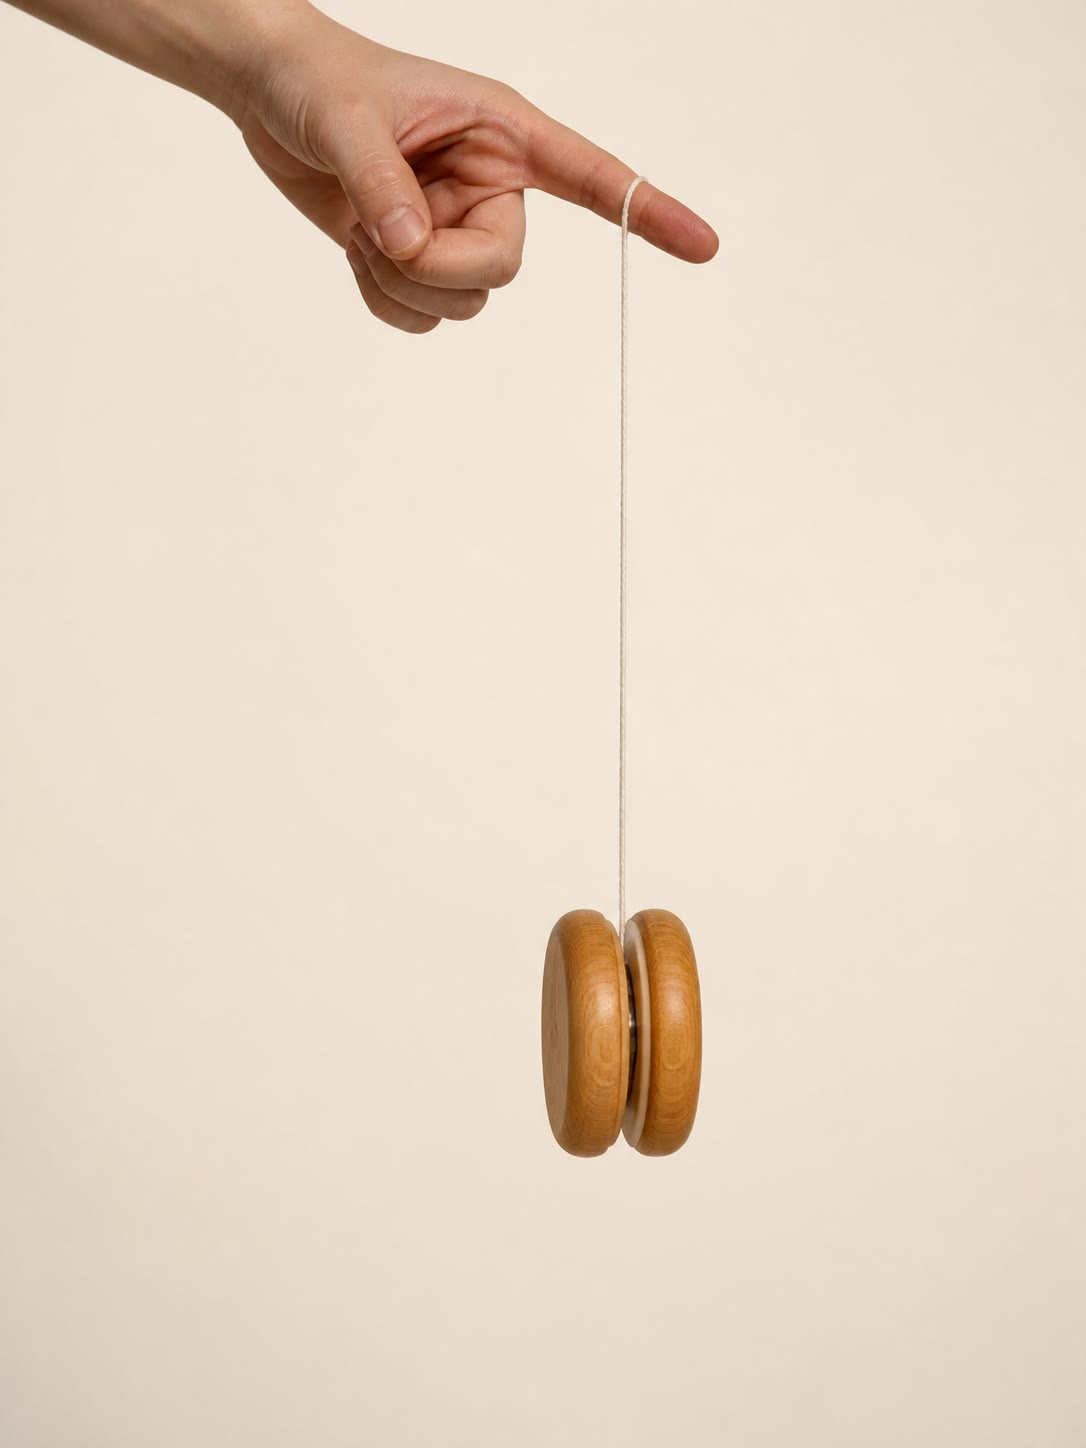
\includegraphics[width=0.34\linewidth]{images/book3/ai/b3-19-yoyo-unwinding.jpg}

{\small 悠悠球退绕：\omterm{def:b1:systems-of-points:cm}{质心}下落，圆盘自转，绳子的张力将两种运动联系起来——周末问题。}
\end{omfigure}

\section{问题：悠悠球}

\begin{problem}[{周末问题——挂在绳子末端细轴上的圆盘：
为什么下落得如此缓慢，到达底端时转得多快，
为什么它会在那里“沉睡”，以及拉动线头时线轴朝哪一侧
滚动}]
\label{pb:b1:systems-of-points:1}
悠悠球是质量为 $M = \qty{50}{g}$、半径为 $R =
\qty{3.0}{cm}$ 的均匀圆盘，其上带有半径为 $r = \qty{0.40}{cm}$ 的细轴，
绳子绕在细轴上，绳长为 $h = \qty{1.0}{m}$，绳子的上端
固定。取 $g = \qty{9.81}{m/s^2}$；$J = \tfrac12 MR^2$ 为绕
该轴的\omterm{prop:b1:angular-momentum:inertia}{转动惯量}。

\medskip
\noindent\textbf{第一部分——运动学与能量。}
\begin{enumerate}
  \item 悠悠球的\omterm{def:b1:systems-of-points:cm}{质心} $G$ 位于何处？为什么？
  \item 由柯尼希定理证明其\omterm{thm:b1:work-and-energy:ke}{动能}为 $\tfrac12
        Mv_G^2 + \tfrac12 J\omega^2$.
  \item 通过对圆环积分推导 $J = \tfrac12 MR^2$，并计算
        $J$.
  \item 当绳子从细轴上无滑动地退绕时，
        建立 $v_G$ 与 $\omega$ 的关系。
  \item 由此推出 $E_k = \tfrac12 Mv_G^2(1 + R^2/2r^2)$，并计算
        括号中的因子，并作评论。
\end{enumerate}

\medskip
\noindent\textbf{第二部分——下落。}
\begin{enumerate}[resume]
  \item 分析悠悠球所受的力；写出\omterm{def:b1:systems-of-points:cm}{质心}定理
        （取竖直向下为正方向）。
  \item 写出对过 $G$ 的轴的\omterm{def:b1:angular-momentum:L}{角动量}定理
        （哪些力有力矩？）
  \item 结合第 4 问，求加速度 $a_G = g/(1 +
        R^2/2r^2)$；计算它。
  \item 求绳子的张力，并与重力比较。
  \item 求退绕 \qty{1.0}{m} 绳子所用的时间，以及此时的速率；
        并与从同一高度释放的石块比较。
  \item 求到达底端时的\omterm{cor:b1:point-kinematics:circular}{角速度}，分别以 rad/s 与每分钟转数表示。
  \item 将底端的\omterm{thm:b1:work-and-energy:ke}{动能}分为平动\omterm{thm:b1:work-and-energy:ke}{动能}
        与转动\omterm{thm:b1:work-and-energy:ke}{动能}两部分。
  \item 检验能量平衡：比较 $Mgh$ 与
        底端的\omterm{thm:b1:work-and-energy:ke}{动能}，并说明绳子的张力虽然很大，
        却不做功。
\end{enumerate}

\medskip
\noindent\textbf{第三部分——底端：沉睡状态。}
绳子完全退绕后，\omterm{def:b1:systems-of-points:cm}{质心}在几
毫秒内即被制止；悠悠球仍在绳端的环中自转
（“沉睡”）。
\begin{enumerate}[resume]
  \item 为什么\omterm{def:b1:systems-of-points:cm}{质心} $G$ 停止后，自转仍能保持？（用哪条定理，
        以及要使其停转需要哪个力？）
  \item 若\omterm{def:b1:systems-of-points:cm}{质心} $G$ 在
        \qty{5}{ms} 内被制止，估算此过程中的平均张力。
  \item 环与细轴摩擦，摩擦力矩 $\Gamma =
        \qty{1.0e-4}{N.m}$，悠悠球将沉睡多久？
  \item 绳子受到向上的猛拉，使绳子重新缠住细轴，
        自转的悠悠球随即上升。利用能量，
        若无任何损失，它能升至多高？实际上为何
        会更低？
  \item 上升过程中，张力比重力大还是小？
        （看 $a_G$ 的符号。）
  \item 若悠悠球的细轴半径等于 $R$，会发生什么？
        （绳子绕在轮缘上）。求其下落加速度。
\end{enumerate}

\medskip
\noindent\textbf{第四部分——桌面上的线轴。}
同一物体放在粗糙的桌面上，细轴水平，
绳子从细轴的\emph{底部}水平引出，
以力 $F$ 拉动，物体无滑动地滚动。
\begin{enumerate}[resume]
  \item 求线轴材料在与桌面接触点 $C$ 处的速度；
        由此推出：每一时刻的运动都是
        绕 $C$ 的转动。
  \item 计算 $F$ 对 $C$ 点的力矩（\omterm{def:b1:angular-momentum:moment}{力臂}为 $R - r$），以及
        重力和桌面反作用\omterm{def:b1:angular-momentum:moment}{力的力矩}。
  \item 利用对 $C$ 的\omterm{def:b1:angular-momentum:L}{角动量}定理，取 $J_C = J +
        MR^2$（惠更斯），求 $a_G$，并证明线轴
        \emph{朝向}手的一侧滚动。
  \item 若绳子以高于水平方向 $\beta$ 角的方向被拉动，
        证明当力 $F$ 的作用线
        通过 $C$ 时线轴不滚动，即 $\cos\beta = r/R$，
        且拉动角度更陡时线轴背离手的一侧滚动，并求出该角度。
  \item 计算 $a_G$，其中 $F = \qty{0.20}{N}$ 为水平拉力，
        并求所需的摩擦力；在线轴开始滑动之前，
        什么因素限制了 $F$ 的大小？
  \item 总结：所用的三条定理（\omterm{def:b1:systems-of-points:cm}{质心}定理，对轴的\omterm{def:b1:angular-momentum:L}{角动量}定理，
        能量定理），以及每条定理所确定的内容。
\end{enumerate}
\end{problem}
